\chapter{2023/12/06}\label{20231206}

\emph{本科教育应给同学们``发现美的眼睛''。}

\emph{GNoME (AI): (11.29 ``Nature'')
发现220万晶体模型,如果人类来做可能需要800年}

\section{SHO again
再谈简谐振子}\label{sho-again-ux518dux8c08ux7b80ux8c10ux632fux5b50}

\subsection*{(1) The phase space of SHO
简谐振子的相空间}\label{the-phase-space-of-sho-ux7b80ux8c10ux632fux5b50ux7684ux76f8ux7a7aux95f4}

We can express \((x, p)\) in phase space (相空间):

The energy of a SHO is the sum of its potential energy and kinetic
energy: \[E = {1 \over 2} kx^2 + {p^2 \over 2m}.\]

Write let the left-hand side be \(1\), and we have
\[{p^2 \over 2mE} + {x^2 \over 2E / k} = 1,\] which is an ellipse
(椭圆).

According to this we have \textbf{phase flow (相流)} and \textbf{phase trajectory (相轨道)}.

\begin{center}
    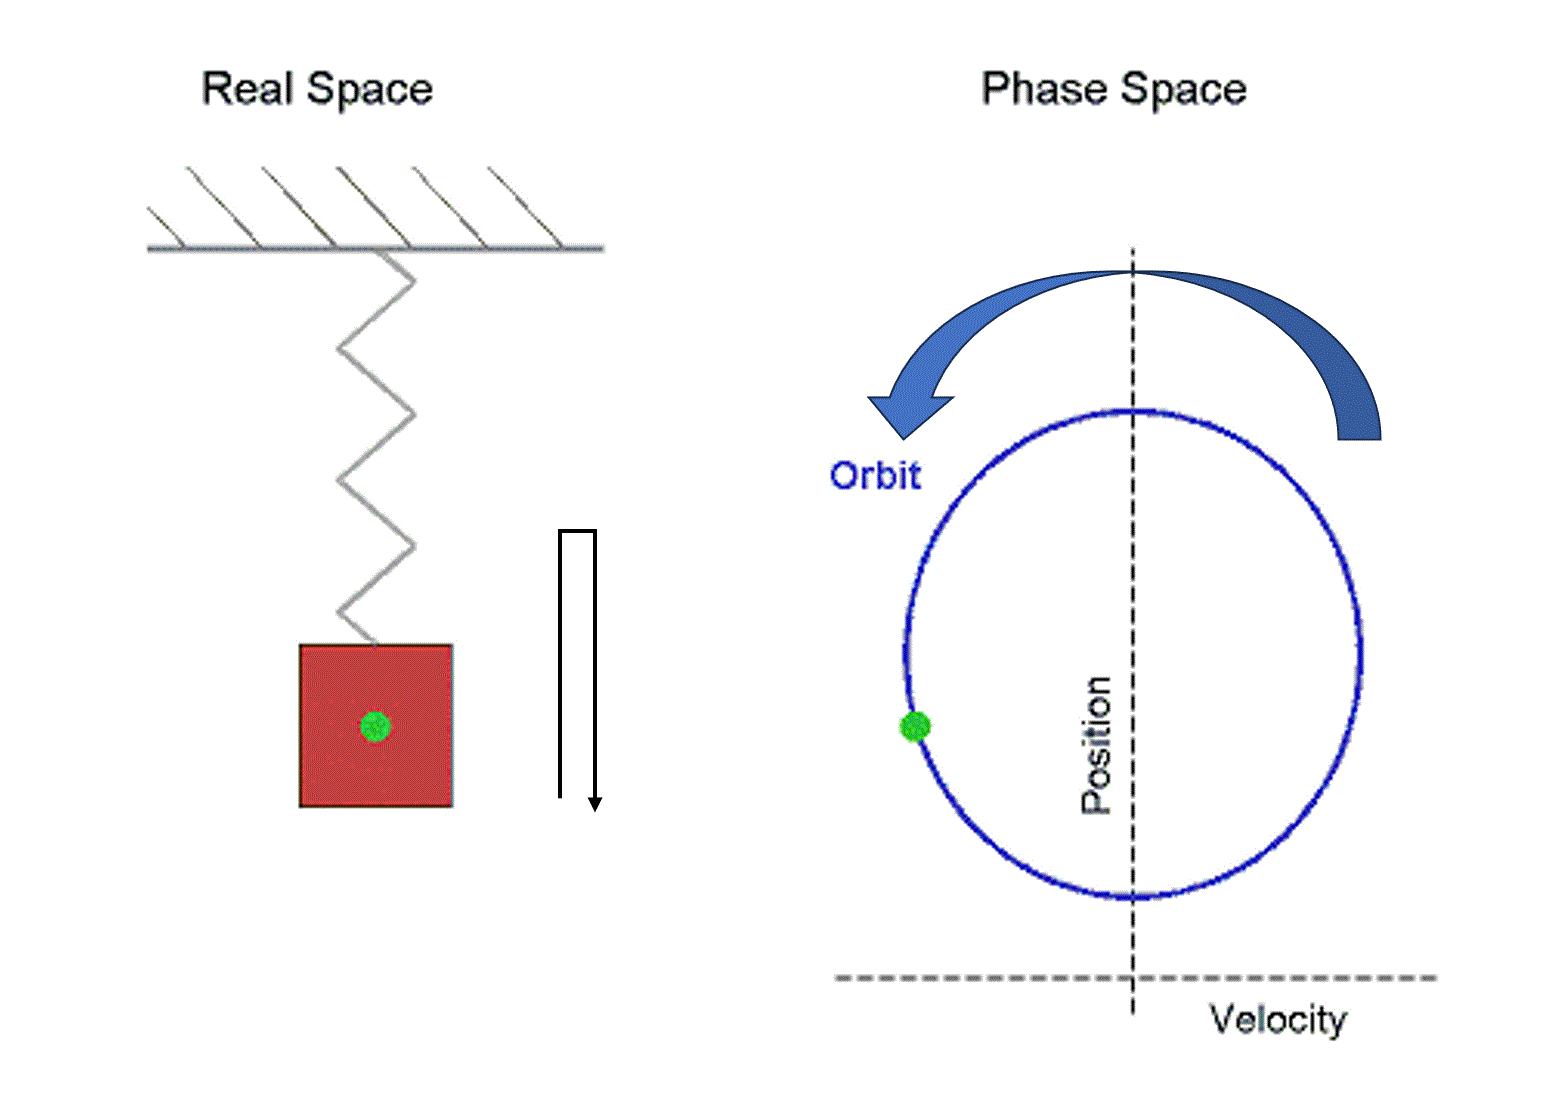
\includegraphics[height=180pt]{assets/Simple_Harmonic_Motion_Orbit.png}
    \captionof{figure}{Phase space of SHO}
\end{center}

\subsection*{(2) Using boundary conditions to find a solution
用边界条件计算简谐振子的解}\label{using-boundary-conditions-to-find-a-solution-ux7528ux8fb9ux754cux6761ux4ef6ux8ba1ux7b97ux7b80ux8c10ux632fux5b50ux7684ux89e3}

The basic function is \(\ddot{x} + \omega_0^2 x = 0\). Its general
solution is \[x = C_1 \cos \omega_0 t + C_2 \sin \omega_0 t.\]

To figure out the values of \(C_1\) and \(C_2\), we need boundary
conditions (边界条件) (for example, initial conditions), for example,
when \(t = 0\), \(x = x_0\) and
\(\displaystyle \frac{\mathrm{d}x}{\mathrm{d}t} = 0\).

In this scenario, when \(t = 0\):
\begin{itemize}
    \item \(x = C_1 = x_0\);
    \item \(\displaystyle \left. \frac{\mathrm{d}x}{\mathrm{d}t} \right|_{t = 0} = - \omega_0 C_1 \sin \omega_0 t + \omega_0 C_2 \cos \omega_0 t \Big|_{t = 0} = C_2 \omega_0 = 0\).
\end{itemize}

That is, \(C_1 = x_0\), and \(C_2 = 0\).

From \(C_2 = 0\), we can simplify \(x\) to \[x = x_0 \cos \omega_0 t.\]
Thus, we have
\[\frac{\mathrm{d}x}{\mathrm{d}t} = - \omega_0 x_0 \sin \omega_0 t\] and
\[\frac{\mathrm{d}^2 x}{\mathrm{d}t^2} = - \omega_0^2 x_0 \cos \omega_0 t = - \omega_0^2 x,\]
where \(\displaystyle \omega_0 = \sqrt{k \over m}.\)

\subsection*{(3) A general method to calculate the
equation of motion of a particle with known potential energy \(U(x)\)
and conserved energy \(E\)
解已知势能和守恒的总能量的质点的运动方程的一种通法}\label{a-general-method-to-calculate-the-equation-of-motion-of-a-particle-with-known-potential-energy-ux-and-conserved-energy-e-ux89e3ux5df2ux77e5ux52bfux80fdux548cux5b88ux6052ux7684ux603bux80fdux91cfux7684ux8d28ux70b9ux7684ux8fd0ux52a8ux65b9ux7a0bux7684ux4e00ux79cdux901aux6cd5}

The general method (under any given potential energy \(U(x)\)) is:
\[E = {1 \over 2} m \dot{x}^2 + U(x).\] From this, we can get
\[\frac{\mathrm{d}x}{\mathrm{d}t}  = \pm \sqrt{\frac{2}{m}[E - U(x)]}.\]
Integrate this, we can get
\[\int_{0}^{t} \mathrm{d}t = \int_{x_0}^{x} \pm \frac{\mathrm{d}x}{\sqrt{\dfrac{2}{m}[E - U(x)]}},\]
from which we can acquire the equation of motion.

\textbf{An example of using this method to solve the equation of motion
of SHO 用这种方法解出简谐振子方程的示例:}

In the particular case of SHO, we know the energy of the particle is
\[E = {1 \over 2} k x_0^2\] and the potential energy is
\[U(x) = {1 \over 2} k x^2.\]

Substitute \(E\) and \(U(x)\) in the equation above, and we have
\[\int_{0}^{t} \mathrm{d}t = \int_{x_0}^{x} \pm \frac{\mathrm{d}x}{\sqrt{\dfrac{2}{m}\left( \dfrac{1}{2} k x_0^2 - \dfrac{1}{2} k x^2 \right)}} = \int_{x_0}^{x} \pm \frac{\mathrm{d}x}{\omega_0 \sqrt{\left( x_0^2 - x^2 \right)}}\]
\[t = \pm {1 \over \omega_0} \arccos \left( {x \over x_0} \right)\]
\[\cos (\mp \omega_0 t) = {x \over x_0}\]
\[x = x_0 \cos \left( \mp \omega_0 t \right) = x_0 \cos \omega_0 t,\]
which is the equation of motion of the SHO.

\subsection*{(4) Series expansion of the equation of motion of the SHO
简谐振子运动方程的级数展开}\label{series-expansion-of-the-equation-of-motion-of-the-sho-ux7b80ux8c10ux632fux5b50ux8fd0ux52a8ux65b9ux7a0bux7684ux7ea7ux6570ux5c55ux5f00}

The basic form of the series expansion of \(x(t)\) is
\[x(t) = a_0 + a_1 t + a_2 t^2 + \cdots + a_n t^n + \cdots = a_0 + \sum_{i = 1}^{\infty} a_i x^i.\]

When \(t = 0\), \(x = x_0\), and therefore \(a_0 = x_0\).

Take the first derivative of \(x\), and we get
\[\frac{\mathrm{d}x}{\mathrm{d}t} = a_1 + 2a_2 t + \cdots + n a_n t^{n - 1} + \cdots.\]

When \(t = 0\), \(\displaystyle \frac{\mathrm{d}x}{\mathrm{d}t} = 0\),
and thus \(a_1 = 0\).

Take the second derivative of \(x\), and we get
\[\frac{\mathrm{d}^2x}{\mathrm{d}t^2} = 2a_2 + 6 a_3 t + 12 a_4 t^2 + \cdots + n(n - 1) a_n t^{n - 2} + \cdots.\]
Also, we know
\(\ddot{x} = - \omega_0^2 x = - \omega_0^2 \left( a_0 + a_1 t + a_2 t^2 + \cdots + a_n t^n + \cdots \right)\).
Therefore, we have \(6a_3 = - \omega_0^2 a_1\), and \(a_3 = a_1 = 0\).

Take more derivatives of \(x\), and in similar ways, we will know that
\[a_1 = a_3 = a_5 = \cdots = a_{2n + 1} = 0.\]

This conclusion can be verified by the series expansion of the cosine
function:
\[x = x_0 \cos \omega_0 t = x_0 \sum_{n = 0}^{\infty} \frac{(-1)^n x^{2n}}{(2n)!} = x_0 \left( 1 - \frac{x^2}{2} + \frac{x^4}{4!} - \frac{x^6}{6!} + \cdots \right).\]

\begin{quote}
作业:托尔斯泰《战争与和平》中的微积分体现在哪里?

比如人之将死,就是积分到了上限;期末考试积分的是你的所有的60个学时的努力。
\end{quote}

\emph{托尔斯泰的伟大可见一斑。}

\section{Features of an inertial coordinate system
惯性系的特征}\label{features-of-an-inertial-coordinate-system-ux60efux6027ux7cfbux7684ux7279ux5f81}

According to Landau, an inertial coordinate system has 3 aspects:

\begin{enumerate}
\def\labelenumi{\arabic{enumi}.}
\tightlist{} 
\item 
  Space:

  \begin{enumerate}
  \def\labelenumii{(\arabic{enumii})}
  \item
    Homogeneity (homogeneous) 空间同质性
    \[{\partial L \over \partial \boldsymbol{r}_\alpha} = \boldsymbol{0}\]
  \item
    Isotropy (isotropic) 空间各向同性
    \[\boldsymbol{v} \cdot \boldsymbol{v}, \boldsymbol{v}^4, \boldsymbol{v}^6, \cdots, \boldsymbol{v}^{2n}, \cdots \quad L(\boldsymbol{v} \cdot \boldsymbol{v}, t)\]
  \end{enumerate}
\item
  Time: Homogeneity 时间同质性
  \[L(\boldsymbol{v} \cdot \boldsymbol{v})\]
\item
  Simplicity 简单性
\end{enumerate}

\section{Galilean group
伽利略群}\label{galilean-group-ux4f3dux5229ux7565ux7fa4}

\emph{编者注:写这里的时候参考了\url{https://en.wikipedia.org/wiki/Galilean_transformation\#Galilean_transformations}.}

Here we use \((t, \boldsymbol{r})\) to express a general point in
spacetime (时空中任意一点).

The Galilean symmetries can be uniquely written as the composition of a
uniform motion of spacetime, a translation and a rotation:

\begin{enumerate}
\def\labelenumi{\arabic{enumi}.}
\item
  Uniform motion with velocity \(\boldsymbol{V}\)
  (速度为\(\boldsymbol{V}\)的匀速运动变换)

  \[g_1(t, \boldsymbol{r}) = (t, \boldsymbol{r} - \boldsymbol{V}t)\]

  This transformation has 3 dimensions.
\item
  Spatial and time translation (时间和空间平移变换)

  \[g_2(t, \boldsymbol{r}) = (t + \tau, \boldsymbol{r} + \boldsymbol{s})\]

  This transformation has 4 dimensions and is called an \textbf{affine
  transformation} (仿射变换).
\item
  Rotation (旋转变换)

  \[g_3(t, \boldsymbol{r}) = (t, \mathbf{R} \cdot \boldsymbol{r})\]

  This transformation has 3 dimensions.
\end{enumerate}

As a Lie group, the group of Galilean transformations has dimension
\(10 \ (3 + 4 + 3 = 10)\).

The Galilean Group is a highly generalized representation of Newtonian
mechanics. Newtonian mechanics is a group that holds under Galilean
transformations.
(伽利略群是对牛顿力学的高度概括。牛顿力学是伽利略变换不变的群。)
